\chapter{Methode}
\section{De fietssimulatie}
Er wordt een simulatie gemaakt die de toestand van de fiets zo goed mogelijk probeert te benaderen. Er zal geen rekening gehouden worden met het manoeuvreren van de fiets of van tegenwind. Enkel de relevante meetwaarden worden bijgehouden. De simulatie is geparametriseerd om eenvoudig verschillende scenario’s te testen.
\\\\
Het voordeel van de fietssimulatie is de enorme flexibiliteit. Uren aan data kunnen in een moment tijd gegenereerd worden, waardoor het makkelijk is om verschillende tests uit te voeren. Hiervoor moeten slechts enkele instellingen aangepast worden. Het is ook mogelijk om slechts een enkele parameter aan te passen tijdens tests terwijl de rest constant blijft (\textit{ceteris paribus}), wat praktisch onmogelijk is in een veldtest. Omdat de simulatie bovendien een duidelijke referentie genereert voor de FCC (output van het fietsersmodel), kan de performantie van de cadanscontroller op een kwantitatieve manier worden geëvalueerd. Tijdens een veldtest zou de fietser alleen kwalitatief kunnen aangeven of hij of zij de voorspelde cadans goed vind. 
\section{Modelleren van het fietserkoppel}
Het fietserkoppel wordt gemodelleerd als een sinusfunctie met twee pieken per omwenteling van de trapas (2 benen), met het DC koppel van de fietser als parameter.
\\
\begin{gather*}
 T_{cy} = T_{dc}(1+sin(2\theta_{cr}-\frac{\pi}{6}))
\end{gather*}
\\
Uit deze formule is het ook meteen duidelijk dat het DC koppel ook het vermogen-equivalent koppel is. Dat wil zeggen dat het DC koppel gedurende een volledige omwenteling van de trapas evenveel arbeid levert als het fietserkoppel.
\\
\begin{align*}
\int_{0}^{2\pi} T_{cy}(1+sin(2x-\frac{\pi}{6})) dx &= T_{cy} \int_{0}^{2\pi}(1+sin(2x-\frac{\pi}{6})) dx\\
&= T_{cy} \left[x-\frac{1}{2}sin(\frac{1}{3}(6x+\pi))\right]_0^{2\pi}\\
&= 2\pi \ T_{cy}
\end{align*}
\\
Het gemiddelde koppel geleverd door de fietser wordt gemodelleerd als een proportionele regelaar. Het doel is om een bepaalde snelheid, $v_{ref}$, te behalen. Hoe groter het verschil is tussen de referentie snelheid en de eigenlijke snelheid, hoe meer kracht er geleverd zal worden. Als deze referentie snelheid overschreden wordt, dan zal er geen koppel meer geleverd worden. Dit wordt ook wel freewheelen genoemd. Om de kracht van de actor te limiteren, wordt er een maximum koppel ingesteld naar gelang de huidige cadans (\gls{omega_cr}). Zo wordt er meer kracht geleverd wanneer de cadans laag is, net zoals in de werkelijkheid. \gls{k} bepaalt de agressiviteit van de regelaar. De formules zien er als volgt uit:

\begin{gather*}
T_{dc,max} = \frac{-\omega_{cr}}{2}+60 \tab (Figuur\ \ref{fig:koppeltoerentalkarakteristiek}) \\
T_{dc} = min(T_{dc,max},max(0,-K*(v_{bike}-v_{ref}))
\end{gather*}
\\
\begin{figure}
  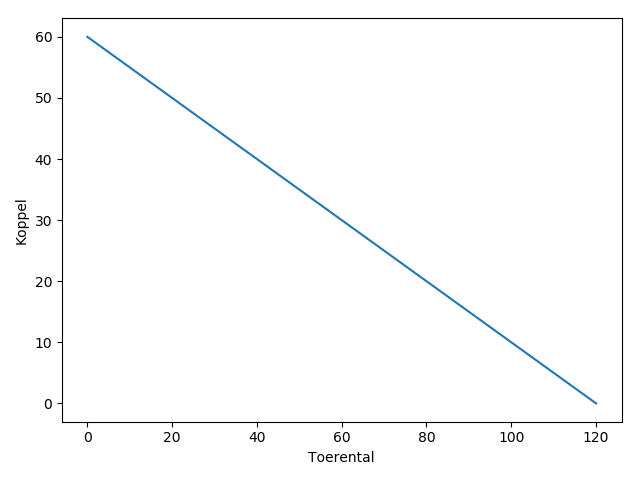
\includegraphics[width=\linewidth]{images/koppel-toerentalkarakteristiek.png}
  \caption{Het koppel-toerentalkarakteristiek}
  \label{fig:koppeltoerentalkarakteristiek}
\end{figure}

Figuren \ref{fig:menselijkkoppelverloop} en \ref{fig:gesimuleerdkoppelverloop} tonen een menselijk koppelverloop en gesimuleerd koppelverloop, gesampled aan 10Hz. Zoals te zien is het gesimuleerde koppel heel consistent. Het menselijk koppel volgt duidelijk een cyclische functie, maar toont vormen van inconsistentie. Merk wel op dat er telkens een afwisseling is van een hoge en een lage piek. Dit wijst op een dominant been. Figuur \ref{fig:gesimuleerde koppel dominant been} toont een gesimuleerd koppelverloop van een fietser met een dominant been.
\\\\
\begin{figure}[t!]
\centering
\begin{subfigure}{.5\textwidth}
  \centering
  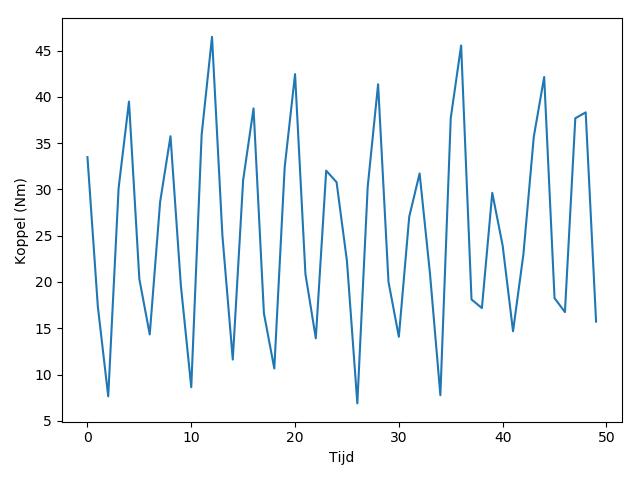
\includegraphics[width=\linewidth]{images/menselijkkoppel.png}
  \caption{Menselijk koppelverloop}
  \label{fig:menselijkkoppelverloop}
\end{subfigure}%
\begin{subfigure}{.5\textwidth}
  \centering
  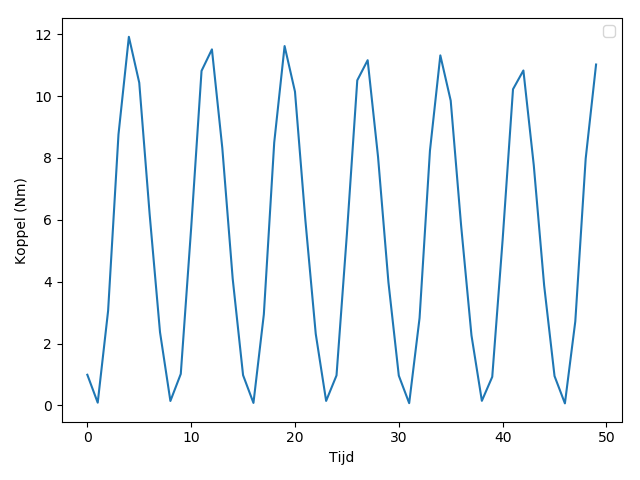
\includegraphics[width=\linewidth]{images/gesimuleerdekoppel.png}
  \caption{Gesimuleerd koppelverloop}
  \label{fig:gesimuleerdkoppelverloop}
\end{subfigure}
\begin{subfigure}{.5\textwidth}
  \centering
  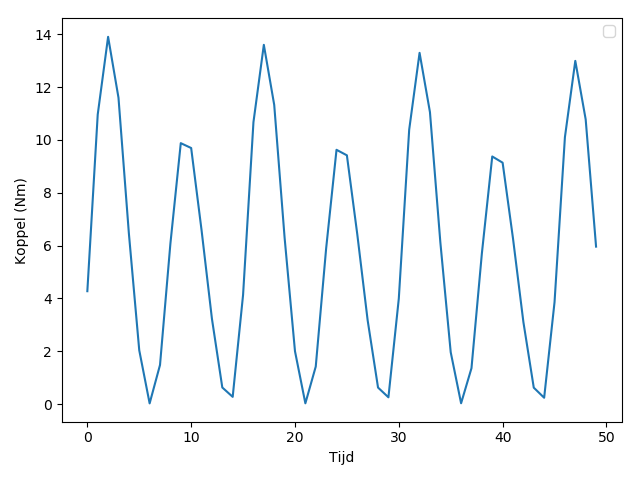
\includegraphics[width=\linewidth]{images/gesimuleerdekoppeldominantbeen.png}
  \caption{Gesimuleerd koppelverloop met dominant been}
  \label{fig:gesimuleerde koppel dominant been}
\end{subfigure}
\caption{Het koppelverloop van een mens (linksboven), de simulatie (rechtsboven) en een gesimuleerd dominant been (onderaan)}
\label{fig:test}
\end{figure}
\newpage
\begin{wrapfigure}{R}{0.5\textwidth}
  \centering
  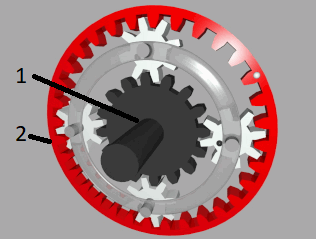
\includegraphics[width=\linewidth]{images/planeetwielmechanisme.png}
  \caption{Planeetwielmechanisme (bron: wikipedia)}
  \label{fig:planeetwielmechanisme}
\end{wrapfigure}

\noindent $T_{cy}$ is het koppel op de trapas. Dit moet nog overgebracht worden op het achterwiel. CoSaR maakt gebruik van een planeetwielmechanisme (figuur \ref{fig:planeetwielmechanisme}). Dit mechanisme laat toe om een grote overbrengingsverhouding te voorzien in een kleine ruimte. Het achterwiel-koppel wordt beïnvloed door het aantal tanden op het zonnewiel (1; \gls{ns}) en het ringwiel (2; \gls{nr}) en de overbrengingsverhouding tussen de trapas en het ringwiel (\gls{k_cr,r}). Het koppel op het achterwiel (\gls{t_rw}) ziet er als volgt uit:
\begin{gather*}
T_{rw}=T_{cy}*k_{cr,r}*\frac{nr+ns}{nr}
\end{gather*}
\\\\
Bovenop het vermogen geproduceerd door de fietser, levert CoSaR extra ondersteuning a.d.h.v. een motor (\gls{t_mg2}) gekoppeld aan het voorwiel. De fietser kan zelf een ondersteuningsniveau (\gls{s}) instellen tussen 0 en 5. Hoe hoger dit ondersteuningsniveau, hoe minder inspanning de fietser moet leveren. 
\begin{gather*}
T_{MG2}=min(35,S\thinspace .\thinspace T_{cy})
\end{gather*}

\section{Het fietsersmodel}
Hoe kiest een fietser zijn cadans? Dit is voor elke fietser verschillend en er is nog nauwelijks onderzoek naar gebeurd. Wielrenners trainen om sneller te kunnen trappen omdat dit efficiënter is.. Ze kunnen een gemiddeld vermogen leveren van 300 Watt. De doorsnee fietser levert gemiddeld ongeveer 75 Watt tijdens een normale fietstocht. Het fietsersmodel zal hierop worden afgesteld, aangezien wielrenners niet de voornaamste doelgroep zijn voor CoSaR.
\\\\
Het fietsersmodel is een functie die op verschillende manieren uitgedrukt kan worden: op basis van de helling, gemiddeld koppel, of een stabiel vermogen. Wat het correcte model is wordt in deze thesis niet uitgewerkt. Het is vooral van belang dat de cadanscontroller het model zo snel en zo nauwkeurig mogelijk kan achterhalen, ongeacht wat het model precies is. Hier wordt de volgende aanname gemaakt: hoe hoger het koppel geleverd door de fietser, hoe hoger de gewenste cadans. Wanneer de fietser bijvoorbeeld een helling oprijdt schakelt hij of zij een versnelling omlaag zodat de kracht die op de pedalen gezet moet worden aangenaam blijft. We stellen hier volgende eenvoudige modellen voor:
\phantom{\gls{f_k}\gls{f_h}\gls{f_v}}
\begin{align*}
Gemiddeld \ koppel:\tab fcc &= f_k . T_{dc}\\
Helling:\tab fcc &= f_h . \alpha\\
Snelheid:\tab fcc &= f_v . v_{bike}
\end{align*}
Er wordt verder aangenomen dat de fietser ook een zeker lineariteit verwacht bij lage snelheden. Dat wil zeggen dat een fietser het niet comfortabel vindt wanneer hij of zij snel moet trappen wanneer de fiets nog stilstaat of heel traag rijdt, ook al moet er op dat moment veel koppel geleverd worden om te kunnen vertrekken. Daarom wordt bij lage snelheden de FCC begrensd door een lineair oplopend maximum, te vergelijken met een mechanische fietsversnelling. Omdat de doorsnee fietser niet heel traag of heel snel trapt wordt de FCC begrensd tussen de 40 en 120 rpm.
\begin{figure}
  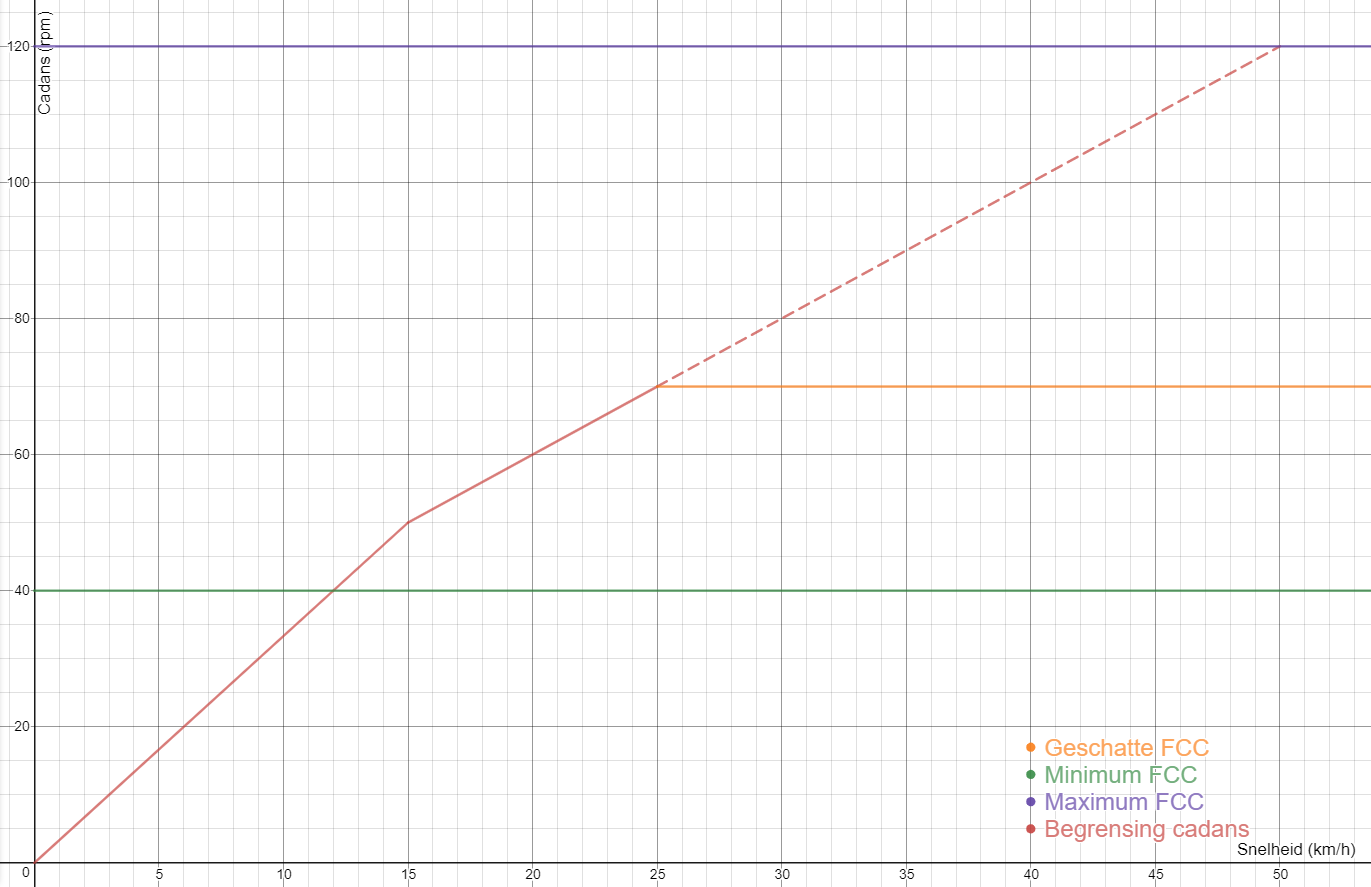
\includegraphics[width=\linewidth]{images/cadansverloop.png}
  \caption{Verwacht cadansverloop in functie van de snelheid. Er wordt verwacht dat de eigenlijke cadans tussen het minimum en maximum ligt.}
  \label{fig:cadansverloop}
\end{figure}
\newpage
\section{Het lastmodel}
De simulatie is voorzien van een lastmodel. Zoals in realiteit, werken lasten in op de fiets. Zwaartekracht, wrijving met de weg en luchtweerstand zijn gemodelleerd als volgt:
\\
\begin{align*}
F_{grav}&=m \ . \ g \ . \ sin \ \alpha \\
F_{friction}&=m \ . \ g. \ c_r \ . \ cos \ \alpha \\
F_{aero}&=\frac{c_d \ . \ \rho_{aero} \ . \ A_{aero} \ . \ v_{bike}^2}{2}
\end{align*}
Samen vormen ze de totale belasting op de fiets, die kwadratisch is in de snelheid.\vphantom{\gls{f_grav}\gls{f_friction}\gls{f_aero}\gls{m}\gls{g}\gls{c_r}\gls{c_d}\gls{rho_aero}\gls{a_aero}\gls{f_load}}
\[F_{load} = F_{grav}+F_{friction}+F_{aero}\]
Deze lasten zorgen ervoor dat de simulatie een realistische hoeveelheid vermogen nodig heeft om een bepaalde snelheid te halen. Er wordt hier geen rekening gehouden met de wind. Ten eerste zou dit extra complexiteit toevoegen aan de simulatie. En ten tweede vermoeden we volgende hypothese:
\\\\
\tab De freely chosen cadence hangt af van de hoeveelheid last, van welke bron dan \tab ook, die de gebruiker ondervindt en de gebruiker zelf.
\\\\
Het voorgestelde lastmodel omvat deze vereiste. Door de helling en referentie snelheid te variëren ondergaat de fietser een veranderende last. Zoals in de realiteit zoeken mensen een bepaalde snelheid te halen. Wanneer de fietser een te hoge last ondervindt, bijvoorbeeld door een berg op te rijden, moet hij of zij meer vermogen genereren om zijn of haar gewenste snelheid te behouden. Hiervoor zijn 2 mogelijkheden: het verhogen van het koppel of de trapsnelheid. Mensen zijn meer geneigd om hun gewenste cadans te behouden, ongeacht het koppel (binnen bepaalde grenzen). De formule voor mechanisch vermogen gaat als volgt:
\[P=T_{cy} \ . \omega_{cr} \]
Om het lastmodel correct te laten werken, moet er nog een helling gegenereerd worden. Om veel werk uit te sparen met het uitstippelen van parcours, wordt dit dynamisch gegenereerd met behulp van perlin noise. Perlin noise kan gebruikt worden om willekeurige getallen te genereren waarbij opeenvolgende getallen weinig van elkaar verschillen. Een perfecte kandidaat dus om terrein te simuleren. Om verschillende trajecten te creëren, kan de seed variabele aangepast worden. Een hellingsgraad wordt in de fietswereld vaak percentueel voorgesteld. Deze implementatie heeft echter radialen nodig. De helling zal beperkt worden tussen $\approx$ 0 en 10\% (0 en 0.1 radialen). Ter vergelijking, de Koppenberg heeft een gemiddeld stijgingspercentage van 11.6\%. Het minimum stijgingspercentage is zo gekozen dat de simulatie zo weinig mogelijk gaat freewheelen.
\begin{figure}[b!]
  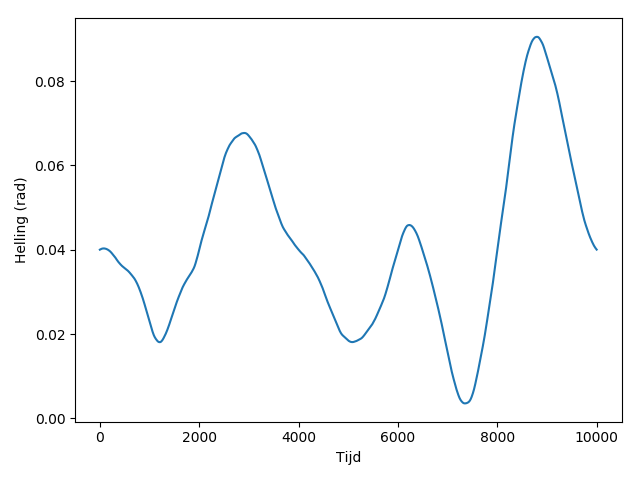
\includegraphics[width=\linewidth]{images/parcour_slope_example.png}
  \caption{Voorbeeld helling verloop}
  \label{fig:hellingverloop}
\end{figure}
\section{Snelheidsvergelijking}
\noindent De snelheid wordt berekend met een standaardformule: vorige snelheid plus acceleratie met respect tot de genomen tijdsprong. De acceleratie is in functie van de last, het totaalgewicht (m), het vermogen geleverd door de fietser op het achterwiel ($T_{rw}$) en het vermogen van een motor bevestigd op het voorwiel ($T_{MG2}$). 
\\\\
De bewegingsvergelijking van de fiets is, met inbegrip van het lastmodel en het fietsersmodel:
\[F \ = \  m \ . \ a \]
Deze vergelijking wordt elke tijdsstap geïntegreerd met behulp van een voorwaartse Euler methode:
\[v_{bike}[h] \ = \ v_{bike}[h-1] \ + \Delta t  \ . \frac{1}{m} \ . \ (\frac{T_{MG2} \ + \ T_{rw}}{r_w} \ - \ F_{load})\]
De volledige simulatie ziet er als volgt uit:
\\\\
 \fbox{\begin{minipage}{\linewidth}
for h in 1..$\#$tijdssprongen\\
\tab $T_{dc,max} = \frac{-\omega_{cr}[h-1]}{2}+60$\\
\tab $T_{dc} = min(T_{dc,max}, \ max(0,-K*(v_{bike}[h-1]-v_{ref}))$\\
\tab $fcc = f(T_{dc})$\\
\tab $\omega_{cr}=cadans(v_{bike}[h-1], \ T_{dc}, \ fcc)$\\
\tab $\theta_{cr}=\theta_{cr}[h-1] + \Delta t \ . \ \omega_{cr}$ \\
\tab $T_{cy} = T_{dc}(1+sin(2\theta_{cr}-\frac{\pi}{6}))$\\
\tab $T_{rw}=T_{cy}*k_{cr,r}*\frac{nr+ns}{nr}$\\
\tab $T_{MG2}=min(35, \ S \ . \ T_{cy})$\\
\tab $F_{grav}=m \ . \ g \ . \ sin \ \alpha$\\
\tab $F_{friction}=m \ . \ g. \ c_r \ . \ cos \ \alpha$\\
\tab $F_{aero}=\frac{c_d \ . \ \rho_{aero} \ . \ A_{aero} \ . \ v_{bike}[h-1]^2}{2}$\\
\tab $F_{load} = F_{grav}+F_{friction}+F_{aero}$\\
\tab $v_{bike} \ = \ v_{bike}[h-1] \ + \Delta t  \ . \frac{1}{m} \ . \ (\frac{T_{MG2} \ + \ T_{rw}}{r_w} \ - \ F_{load})$
\end{minipage}}